% !Mode:: "TeX:UTF-8"

\chapter{红外无人机目标检测算法}

\section{引言}
本课题研究的红外无人机目标检测算法,主要需要解决的问题有两个。
一个是原始图像是由红外设备产生的,因此原始图片是灰度图,
不含有普通BGR图像的三个通道信息;
另一个问题是在实际的检测场景下,无人机目标在检测设备中的成像往往伴随相当复杂的背景,
本课题对算法的复杂背景下目标的检测能力要求较高。
因此本章所做的研究首先是针对本课题的红外无人机目标检测问题
建立研究必要的数据集,
之后选择一种在该数据集上性能较好的深度学习算法
作为基础算法,接着针对上述的两个问题提出了
基于通道填充和图像合成的数据增强算法,
在mAP和推理时间两个方面
进一步提升算法在数据集上的性能表现。

\section{数据集制作}[Number]
由于神经网络需要大量的数据进行训练,
并且算法还需要在数据集上进行测试,
因此本课题研究需要一个红外无人机目标的数据集。
由于目前尚无开源红外无人机数据集可供使用,
本课题自建了红外无人机数据集。

\subsection{数据集概况}
目前国内外完善标注的公开红外数据集很少,
仅有少量红外无人机数据集但多以点标注形式发布,
因此需要自行收集红外无人机图像并进行标注。
考虑到网络模型的泛化能力和特征提取的鲁棒性,
自行收集了多种背景的红外图像,
并且覆盖距离远近的无人机目标,目标全部为旋翼无人机。
数据集来源主要是网络获取和实验室自主采集两种方式,
格式为红外无人机图像和视频,通过脚本转换为图片格式后,
标注目标框,制作成数据集,总共包含10000张图片,原始格式为PASCAL VOC,
按训练集、验证集、测试集划分分别有7000张、2000张、1000张。
数据集中的原图示例如图\ref{dataset}所示。

\begin{figure}[!h]
    \setlength{\subfigcapskip}{-1bp}

    \centering
    \begin{minipage}{\textwidth}
    \centering
    \subfigure{\label{dataset11}}\addtocounter{subfigure}{-2}
    \subfigure{\subfigure[正常目标示例~1]{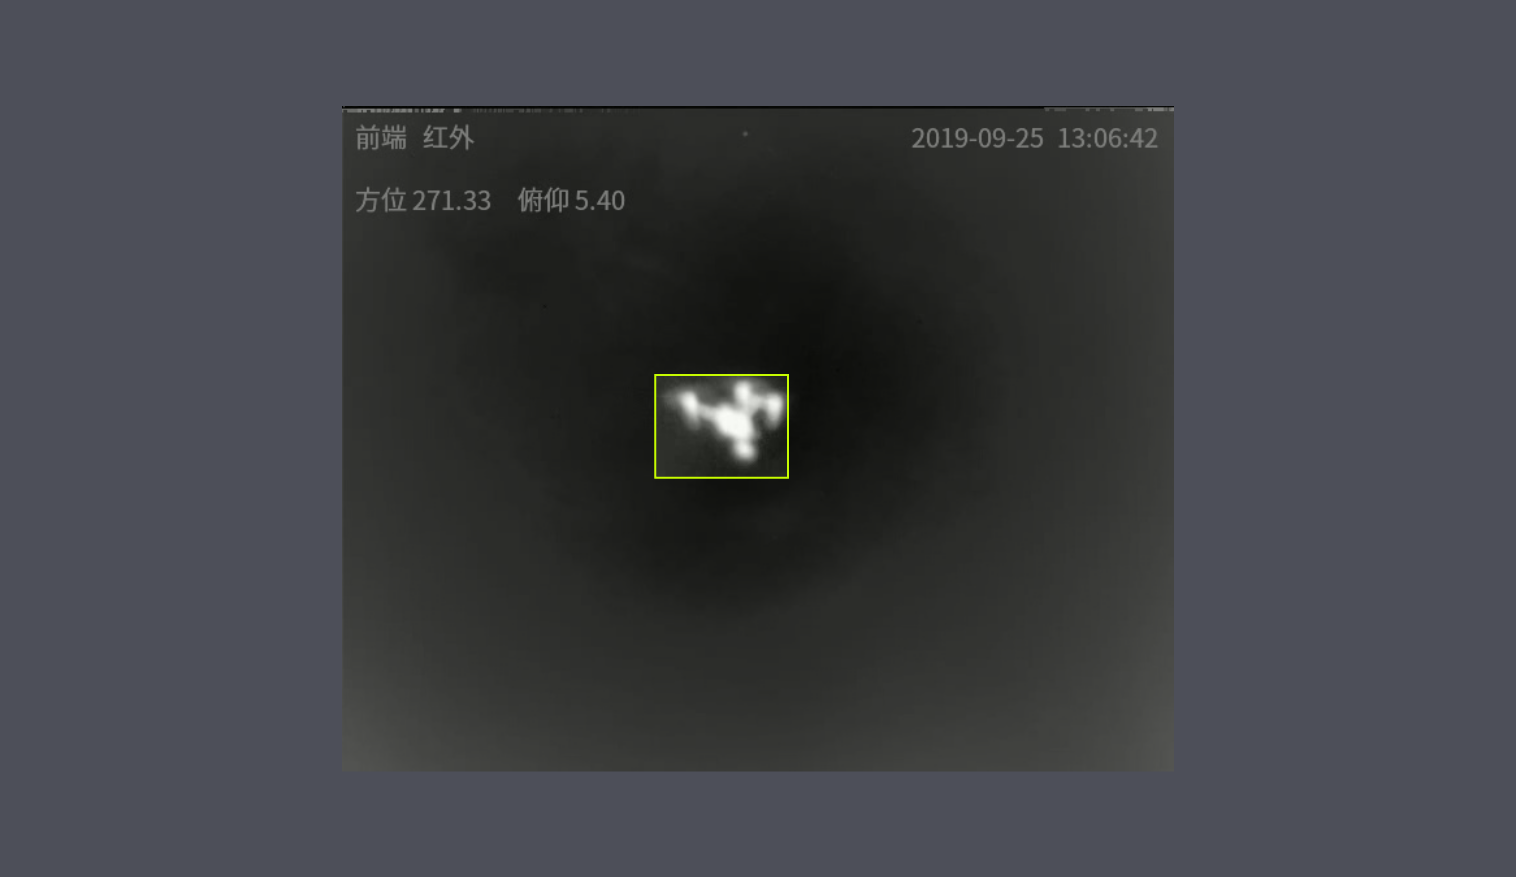
\includegraphics[width=0.4\textwidth]{1.png}}}
    \hspace{2em}
    \subfigure{\label{dataset12}}\addtocounter{subfigure}{-2}
    \subfigure{\subfigure[正常目标示例~2]{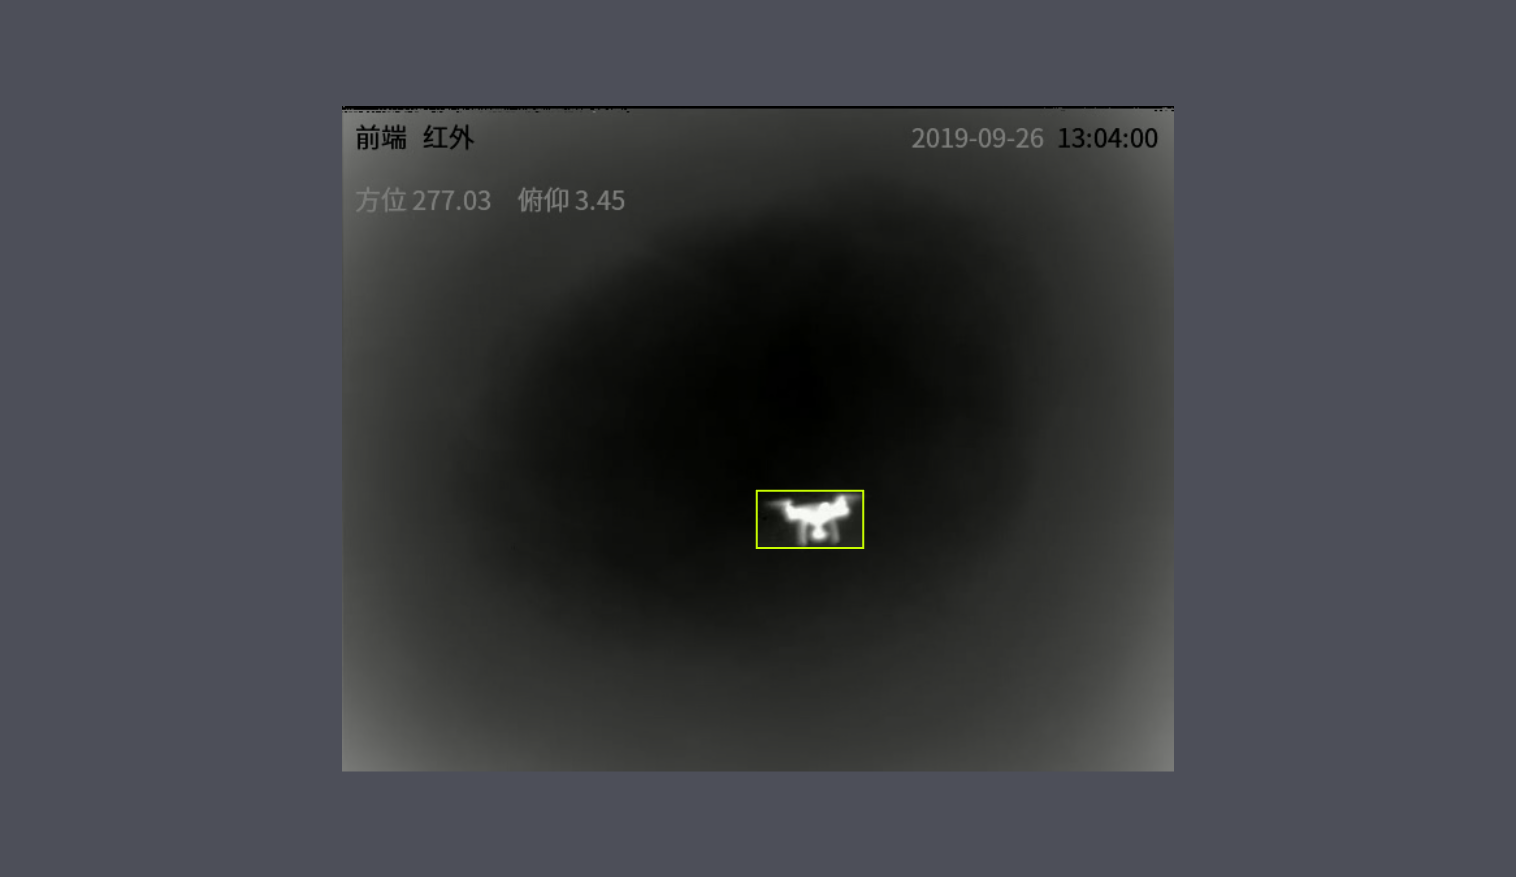
\includegraphics[width=0.4\textwidth]{2.png}}}
    \end{minipage}

    \centering
    \begin{minipage}{\textwidth}
    \centering
    \subfigure{\label{dataset21}}\addtocounter{subfigure}{-2}
    \subfigure{\subfigure[小目标示例~1]{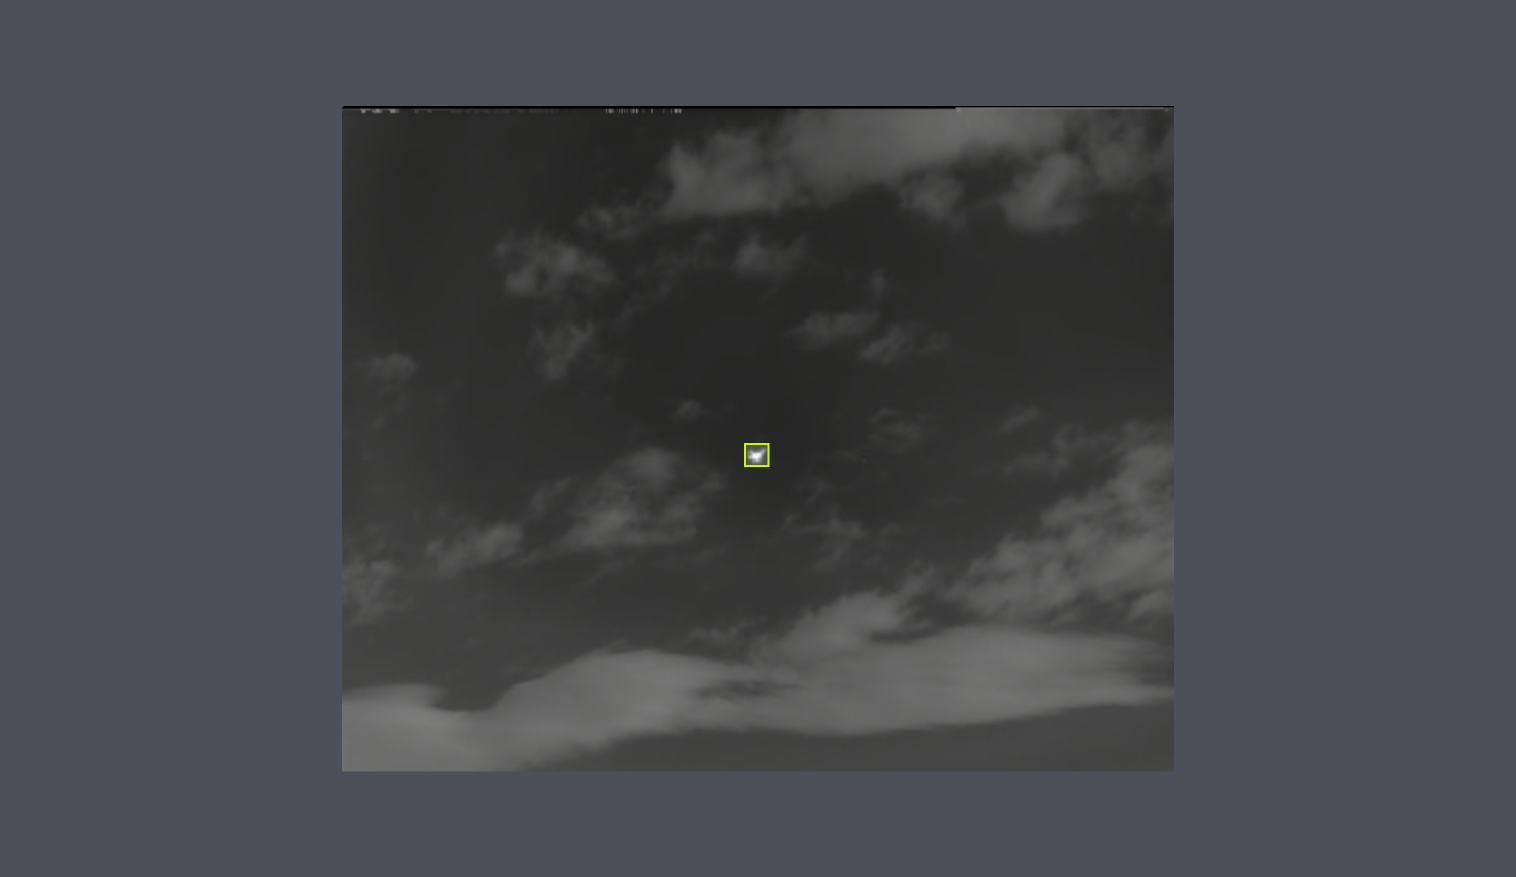
\includegraphics[width=0.4\textwidth]{5.png}}}
    \hspace{2em}
    \subfigure{\label{dataset22}}\addtocounter{subfigure}{-2}
    \subfigure{\subfigure[小目标示例~2]{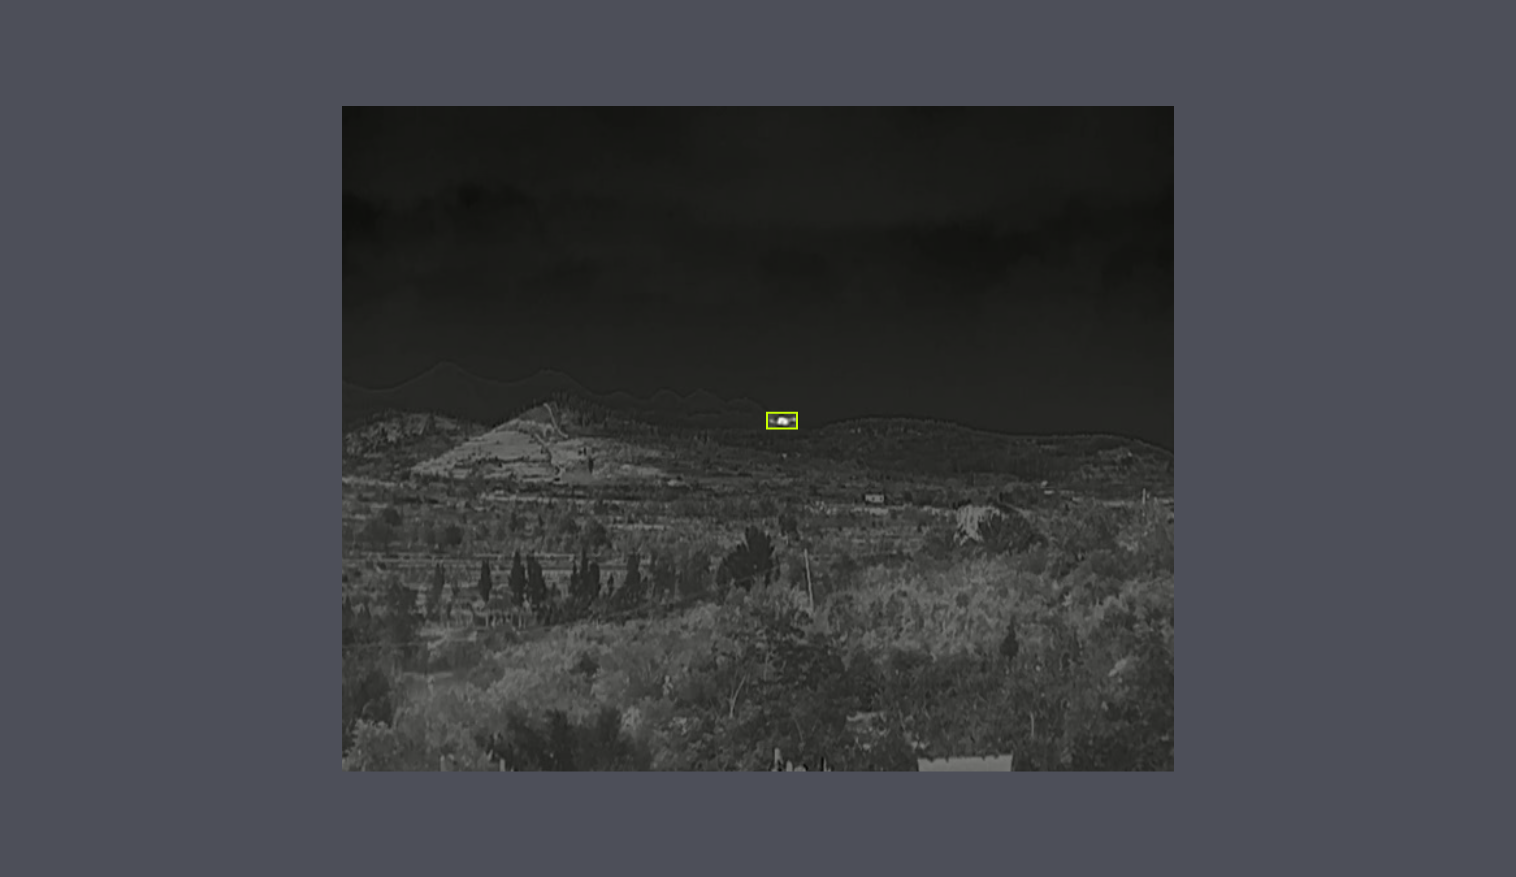
\includegraphics[width=0.4\textwidth]{6.png}}}
    \end{minipage}

    \centering
    \begin{minipage}{\textwidth}
    \centering
    \subfigure{\label{dataset31}}\addtocounter{subfigure}{-2}
    \subfigure{\subfigure[遮挡目标示例~1]{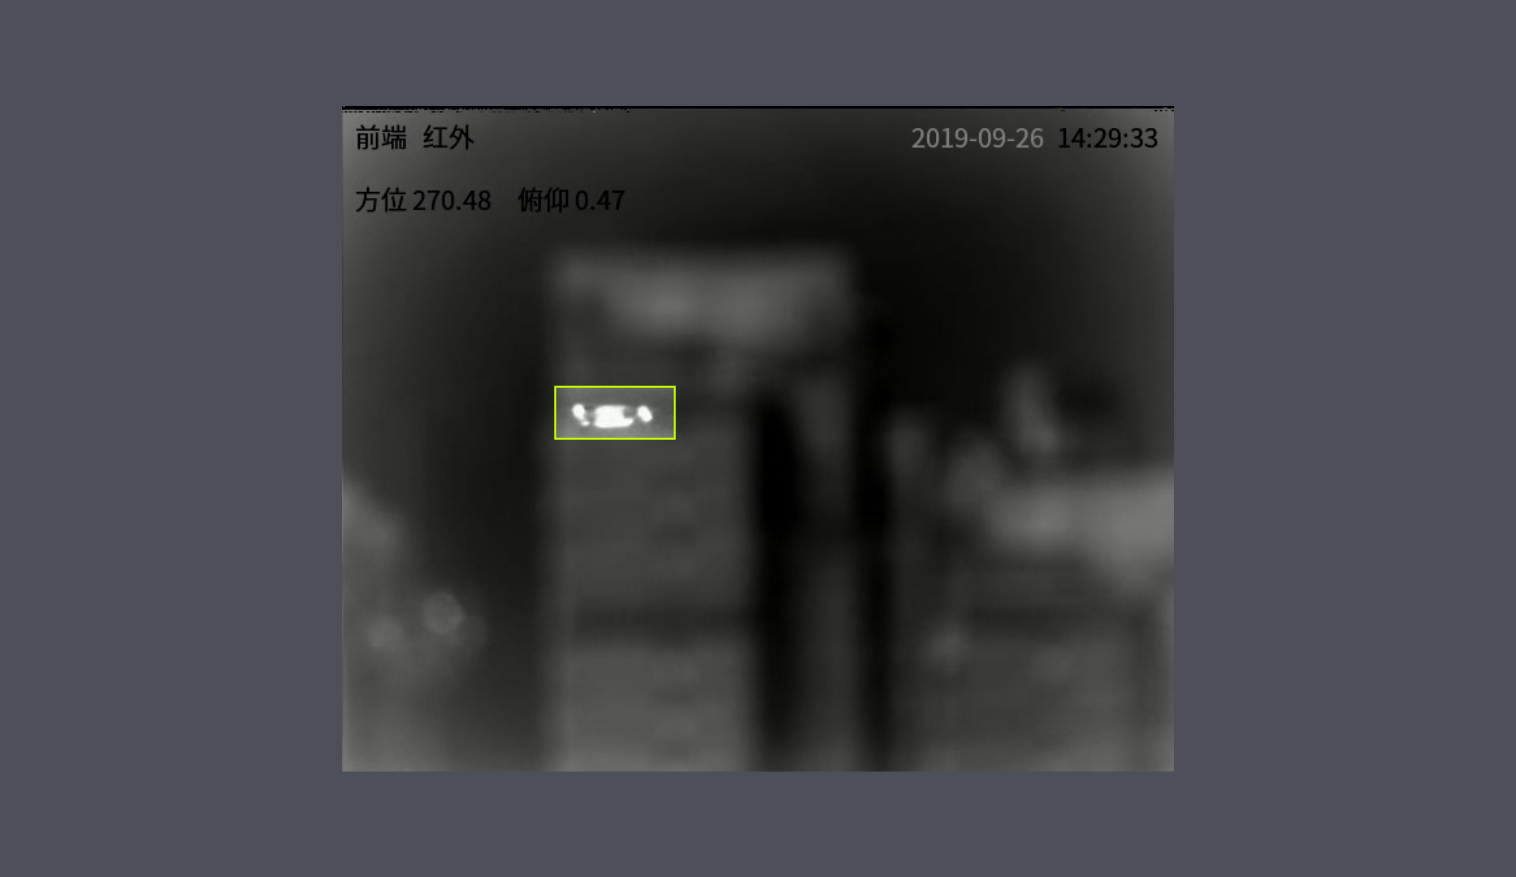
\includegraphics[width=0.4\textwidth]{3.png}}}
    \hspace{2em}
    \subfigure{\label{dataset32}}\addtocounter{subfigure}{-2}
    \subfigure{\subfigure[遮挡目标示例~2]{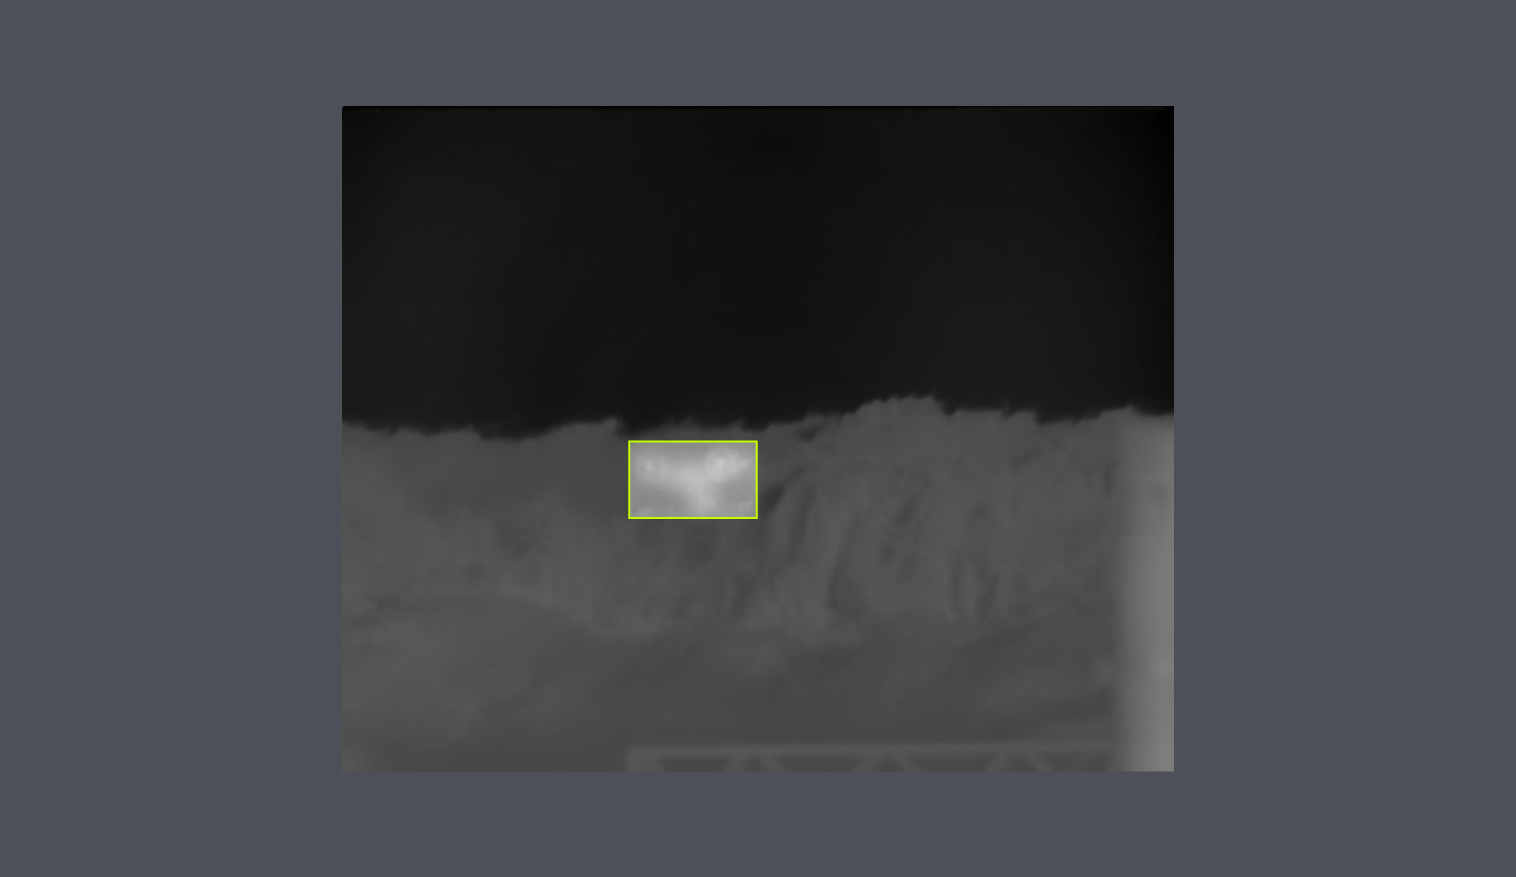
\includegraphics[width=0.4\textwidth]{4.png}}}
    \end{minipage}

    \vspace{0.2em}
    \caption{数据集图像示例}
    {\label{dataset}}
\end{figure}


\section{深度学习网络模型基本算法YOLOv5}
本课题算法的主干网络模型采用YOLOv5网络,网络的结构如图\ref{yolo1}所示,
该模型按照推理流程顺序主要可以分成
输入端、Backbone、Neck、Prediction这四个部分。

\begin{figure}[h]
    \centering
    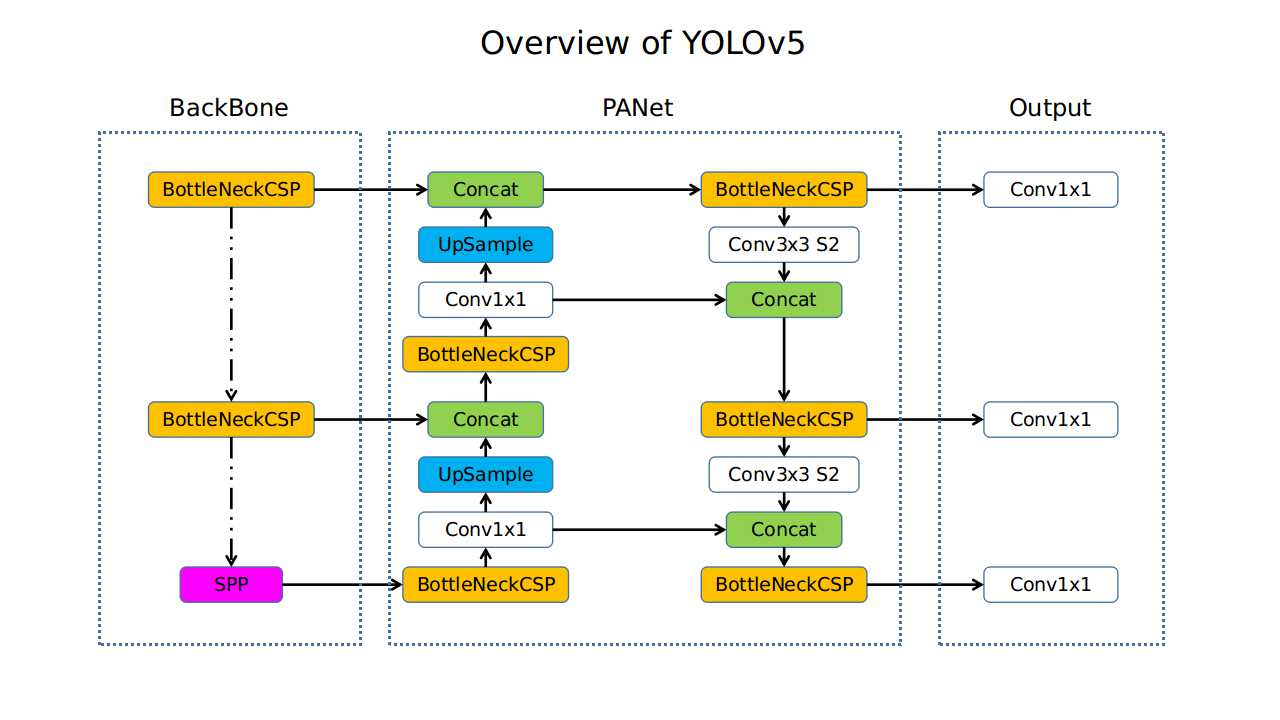
\includegraphics[width = 0.8\textwidth]{yolov5结构.jpg}
    \caption{yolov5网络结构}
    \label{yolo1}
\end{figure}

\subsection{输入端}
YOLOv5网络的输入端就是输入图像的模块,
既可以向网络提供原始的图像输入,
也可以在这个部分对图像进行预处理
和数据增强,
此外还能进行算法的准备工作,比如锚框的
自适应计算等。

\subsection{Backbone}
Backbone的主要作用是初步提取特征图。其中典型的模块是Focus模块、CBL模块以及CSP模块。

\subsubsection{Focus模块}
Focus模块是主要功能是对输入图像进行初步处理,将图像进行切分,以类似降采样的间隔取值方式将原图像中的像素点拆分后组合为新的小图像,这样处理的作用是扩充了输入的通道数,同时没有信息丢失的问题。对于具体的某张输入图像,如果应用$4\times4$规格的Focus切片处理,就可以将输出通道由原本的BGR形式的3个通道扩充到12个通道,每张输出特征图尺寸则会变成输入图像的$\frac{1}{4}$。最后对切分后的图片应用卷积运算。Focus切片处理的过程如图\ref{focus}所示。

\begin{figure}[h]
  \centering
  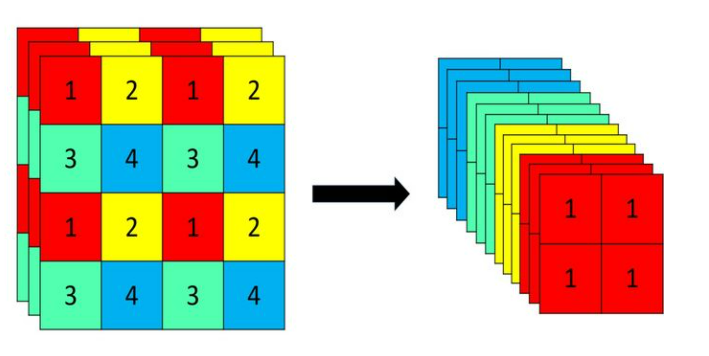
\includegraphics[width = 0.8\textwidth]{focus.png}
  \caption{Focus切片示意图}
  \label{focus}
\end{figure}

\subsubsection{CBL模块}
CBL模块是卷积神经网络的基本组成模式,
结构如图\ref{cbl}所示,
由卷积、归一化、激活函数三个部分组成。
CBL的主要作用是通过卷积采集特征。
其中的激活函数默认是Leaky ReLU,Leaky Rectified Linear Unit是一种基于 ReLU 的激活函数,但它对于负值的斜率很小,而不是平缓的斜率。 斜率系数是在训练之前确定的,即它不是在训练期间学习的。 这种类型的激活函数在我们可能遭受稀疏梯度的任务中很受欢迎。

\begin{figure}[h]
  \centering
  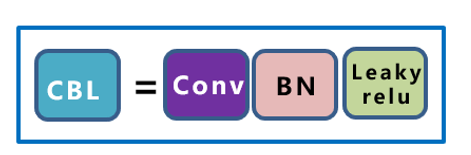
\includegraphics[width = 0.5\textwidth]{CBL.png}
  \caption{CBL模块组成示意图}
  \label{cbl}
\end{figure}

\begin{figure}[h]
  \centering
  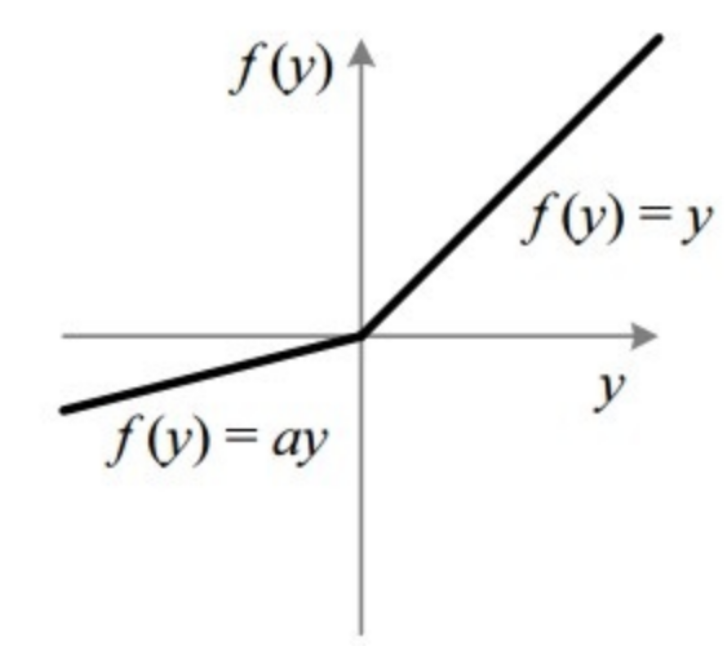
\includegraphics[width = 0.4\textwidth]{leakyrelu.png}
  \caption{Leaky ReLU示意图}
  \label{relu}
\end{figure}

\subsubsection{CSP模块}
CSP模块的主要作用是解决以往的网络推理计算中计算量过大的问题,具体地处理思路是,通过缓解网络计算优化中的过多重复梯度信息的现象来降低网络中过高的计算负载。CSP 模块把输入特征图分割为两部分,并且在后续处理中通过合并的方式兼顾梯度的充分组合和计算量的优化。
YOLOv5网络的Backbone部分采用创新的CSPDarknet,达到提取输入图像的重要特征的目的。CSPDarknet的主要优势在于简化了梯度信息的传递,同时减少了整个YOLOv5算法系统的参数量和计算量。

\begin{figure}[h]
  \centering
  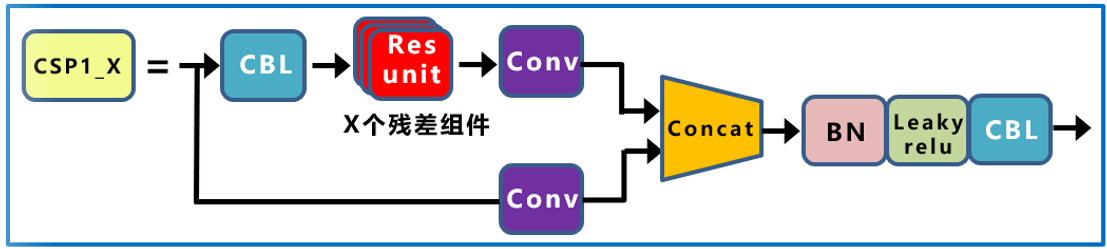
\includegraphics[width = 0.8\textwidth]{CSP.png}
  \caption{CSP模块组成示意图}
  \label{csp}
\end{figure}

\subsection{Neck及Prediction}
Neck部分主要由FPN和PAN组成。FPN指的是特征金字塔网络(Feature Pyramid Network),特征金字塔是一种
用于检测不同尺度物体的系统。该算法模块利用固有的多尺度,
深度卷积网络的金字塔层次结构以边际额外成本构建特征金字塔。研究人员开发了具有横向连接的自上而下的架构,
主要作用是建立各个尺度的语义特征图。这种架构作为通用特征提取器在不同场景均显示出出色的性能。
FPN对小尺度目标检测效果更好。FPN可以利用经过top-down模型后的那些上下文信息(高层语义信息)。
对于小目标而言,FPN增加了特征映射的分辨率(即在更大的feature map上面进行操作,这样可以获得更多关于小目标的有用信息)。

PANet是一种旨在提升信息的路径聚合网络结构(Path Aggregation Network)。
具体来说,PANet增强了整个特征层次结构中
自下而上的低层精确定位信号,提出了自适应特征池,
它将特征网格和所有特征级别联系起来,进而在每个特征级别中生成有用的信息
直接传播到以下提议子网,缩短了较低层和最顶层特征之间的信息路径。
PANet在实例分割和目标检测等任务中均有着优秀的性能表现。

Prediction部分包含上级输出的特征向量,并通过输入的特征向量得出坐标值、置信度,结合损失函数和后处理函数得出检测结果。

\subsection{YOLOv5基础网络性能验证与分析}
本节将在自建数据集上对YOLOv5基础网络的性能进行验证,将其与常见算法SSD和Faster R-CNN进行对比,并分析YOLOv5算法的优势。
为了证明基础YOLOv5算法在红外无人机目标检测任务中的有效性,本节将其与目标检测算法SSD以及Faster R-CNN进行对比实验。
本章提到的YOLOv5基础算法用深度学习网络框架Pytorch进行实现、训练和测试。操作系统为Windows 10,使用的主要软件为python。实验平台采用的CPU型号为Intel Core i7-11700k,GPU型号为NVIDIA GeForce RTX 3080Ti,显存容量为12GB。训练过程中使用GPU进行加速。



\begin{table}[htbp]
  \caption{不同算法对红外无人机数据集的检测结果}
  \vspace{0.5em}\centering\wuhao
  \begin{tabular}{ccc}
  \toprule
  检测算法 & mAP & 推理时间(ms)\\
  \midrule
  Faster R-CNN & 0.625 & 12.5\\
  SSD & 0.705 & 10.3\\
  YOLOv3 & 0.904 & 7.5\\
  YOLOv5 & 0.919 & 2.5\\
  \bottomrule
  \end{tabular}
  \label{t11}
\end{table}

根据表\ref{t11}中的实验结果,Faster R-CNN在本文自建红外图像无人机目标检测数据集的mAP较低,同时会消耗更多的推理时间。这是因为Faster R-CNN算法虽然相对于R-CNN算法有所改进,但是仍然采用二阶段检测方式,先进行提名候选框后进行目标检测,这种检测方式虽然一定程度上保证了检测精度,但是会使得算法总体的检测耗时较长。而SSD算法在单阶段检测的同时,引入了特征金字塔结构,充分利用了多尺度目标的特征,因而能在检测精度和推理时间上都有较好的表现。而YOLOv3由于经过了几次迭代和改进,所以精度上比SSD算法和Faster R-CNN算法更高且检测速度较快。由于YOLO系列算法直接采用了单阶段检测,较大程度地减少了推理时间。但是由于网络结构中没有充分利用多尺度特征信息,因此在尺度变化较大的数据集上精度不高。而YOLOv5网络在YOLOv3的基础上,应用了很多提升精度的改进,如增加了PANet、改进了损失函数等,也应用了很多提升速度的改进,如应用了CSP模块等,因此在实验结果中体现出YOLOv5的检测精度和推理时间都是最优的,因此本文选择YOLOv5算法作为红外无人机目标检测算法的基础。

\section{数据增强算法}
由于深度学习算法通常需要大量的数据进行学习,因此在原始数据集的基础上,将基础网络结合数据增强算法能在一定程度上提升算法的性能。因此本节将对常见的图像增强算法进行实验,在实验结果的基础上针对红外图像目标检测任务提出一种图像填充算法,此外还将针对红外无人机目标检测任务中的背景较为复杂的特性提出一种图像拼接的数据增强算法。

\subsection{主流的图像增强算法}
目前计算机视觉领域常见的图像增强处理算法可以根据对输入图像的处理方式划分为
空域增强算法和频域增强算法。空域指的是图像的像素维度,即对组成原始图像的各个像素直接处理,常见的空域增强方法有降噪、直方图均衡等。
频域指的是图像的频率域,一般包含图像的变化快慢信息。因此频率域的增强往往关注图像的边缘等从频率角度观察会表现得更为直观的信息。
考虑到处理的复杂度和时间成本,本文从空域角度重点研究图像的增强算法。

对输入图像进行空域增强的过程可以定义成如式\ref{aug1}所示:

\begin{equation}
  g(x, y)=T[f(x, y)]
  \label{aug1}
\end{equation}

式中$f(x, y)$代表输入的原始图像,$T$是一种空间域变换的定义,$g(x, y)$表示经过空域增强算法处理后的输出图像。

\subsubsection{Inversion}
由于主流的目标检测算法应用的场景都是基于BGR图像的,不适于检测红外目标,因此需要将红外图像进行预处理以达到使红外图像更接近BGR图像的目的,通过域迁移的思想使得网络能够更加适应处理后的红外图像。一般用于目标检测所用的RGB图像都是白天所摄,通常情况是背景较亮,目标较暗。但是红外图像成像为辐射特性,故一般背景辐射较弱而目标辐射较强。因此,考虑采用Inversion操作对输入的原始图像进行处理,Inversion处理的过程如式\ref{inv1}所示:
\begin{equation}
  f: x_{p}=u-x
  \label{inv1}
\end{equation}

式中,$x_{p}$表示Inversion处理后的输出图像,$u$表示图像系统中像素强度值的上限,特别地,对于8bit色深的图像色彩系统,$u$的值为255。$x$表示输入的原始图像。

\subsubsection{直方图均衡}
通常情况下,红外图像的灰度往往集中在某个值域内,这是因为红外成像系统采集到的图像对比度较低,因此需要运用直方图均衡的算法将输入图像的灰度均匀地分散到更大的范围内,使得图像的整体对比度提升,从而降低后续的目标检测算法的处理难度。
一般情况下,直方图均衡处理算法的过程如下: 

(1)对输入图像,统计其每个像素点的灰度值分布情况,计算方法如式\ref{he1}所示。
\begin{equation}
  \mathrm{p}_{r}\left(r_{k}\right)=\frac{n_{k}}{n} \quad k=0,1,2, \ldots, L-1
  \label{he1}
\end{equation}

其中$n$代表输入图像的像素点总个数,$n_{k}$代表灰度经离散化处理后处于$r_{k}$间隔的像素点个数。

(2)对图像的灰度分布情况,可以得到变换后的图像灰度分布,计算过程如式\label{pix trans}所示:
\begin{equation}
  \mathrm{s}_{k}=T\left(r_{k}\right)=\sum_{j=0}^{k} p_{r}\left(r_{j}\right)=\sum_{j=0}^{k} \frac{n_{j}}{n} \quad k=0,1,2, \ldots L-1
  \label{pix trans}
\end{equation}

通过式\ref{pix trans}
可以获得处理之后像素点的灰度分布情况,其中$r_{k}$表示处理前的像素点灰度值,$s_{k}$表示处理后输出的像素点的灰度值。

直方图均衡是一种常见的提高输入图像对比度的方式,同时还具有计算时间负载较小的优势,但是该算法存在的问题是可能造成图像中细粒度特征的强度降低,针对这个问题后续的研究人员提出了对比度受限的直方图均衡等方法。

\subsubsection{USM锐化}
对于大多数情况下的目标检测任务,目标相对背景都是有较明显的轮廓,因此可以采用锐化处理方法进一步加强物体的边界,进而增强检测效果。

锐化的本质是对原图像实现高通滤波,得到原图像的高频分量,也就是对原图像中的边缘部分进行了增强。计算机视觉图像增强算法中一种性能较好的锐化方法是USM(Unsharp Mask)算法,这种处理方法的主要思想是先获得输入图像中变化较慢的低频分量,之后利用该低通分量对原始图像进行掩模处理,意图是使原始图像消去自身的低频分量后保留高频分量,从而达到锐化图像的目的。
基于USM的锐化算法比直接使用利用算子对输入图像进行卷积的锐化方式应用更加广泛,原因是USM算法一定程度上不会受到较弱的干扰噪声的影响。
\begin{equation}
  I_{sharpend}=I_{original}+(I_{original}-I_{blurred})*a
\end{equation}

式中$I_{sharpend}$表示锐化后的图像,$I_{original}$表示原始图像,$I_{blurred}$表示模糊后的原始图像,$a$表示权重系数。

\subsection{通道填充算法}
本章结合第2章中分析的红外图像的成像特点,认为红外图像存在信息量不足等特点,使得在可见光目标检测领域性能优秀的目标检测算法难以直接通过迁移就取得良好的性能。因此本节中提出了一种基于通道填充的红外图像数据增强算法,核心思想是抓住红外图像和可见光图像之间的主要差异,即红外图像仅有1个灰度通道进行信息的表达,而可见光图像通常包含BGR3个通道,考虑将原始的红外图像由单通道填充为和可见光图像相同的3个通道,增加参与训练的数据量,提高YOLOv5目标检测算法模型的学习效果和检测性能。
通道填充算
法的流程如图\ref{tdtc}所示。

\begin{figure}[h]
  \centering
  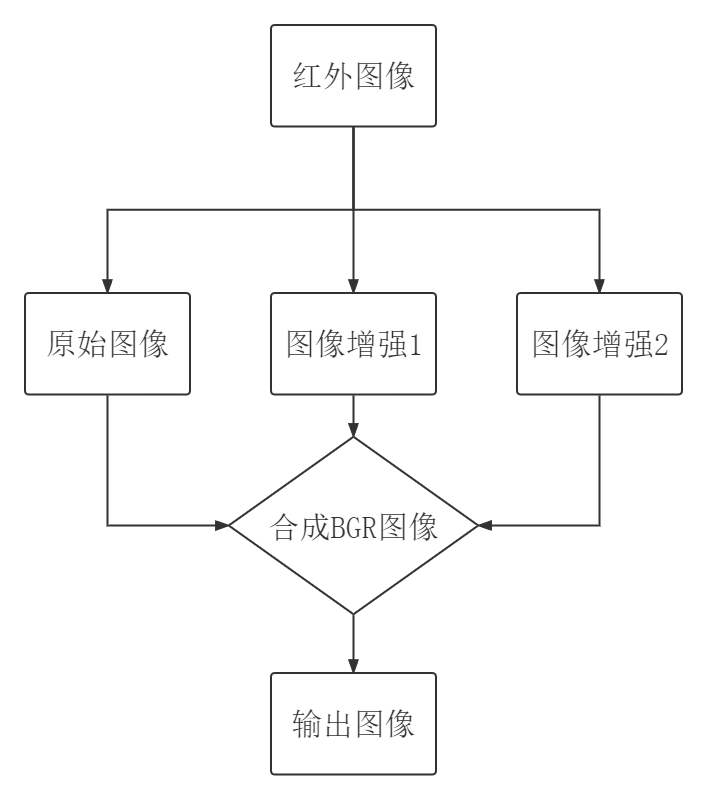
\includegraphics[width = 0.6\textwidth]{通道填充流程图.png}
  \caption{通道填充算法流程图}
  \label{tdtc}
\end{figure}

由于该算法输出的图像包含3个通道,其中1个是原始的红外灰度图像,另外两个通道采用以下3种图像增强算法中的两个,具体选择策略经过实验对比后确定。

(1)Inversion。主要目的在于增强图像的信息多样性,同时使得红外图像更加贴近可见光图像的特性。

(2)CLAHE。主要作用是提升输入红外图像的对比度,和普通HE算法的主要区别是CLAHE算法对整个图像进行分区后再进行HE处理,能更细粒度地起到增强图像对比度的作用。

(3)USM变换。主要目的在于抑制噪声的同时进行图像的锐化,强化目标的边缘。本文使用高斯模糊后的USM变换进行锐化。

\begin{figure}[htbp]
	\centering
	\begin{minipage}{0.49\linewidth}
		\centering
		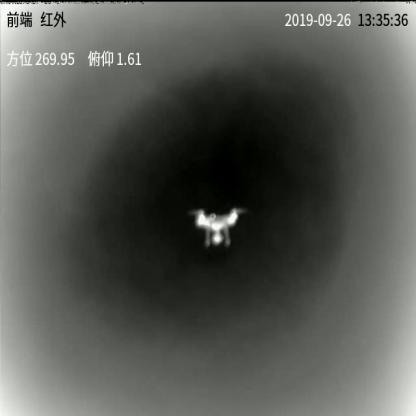
\includegraphics[width=0.9\linewidth]{原图1.JPG}
		\caption{原图示例}
		\label{txzq11}%文中引用该图片代号
	\end{minipage}
	\begin{minipage}{0.49\linewidth}
		\centering
		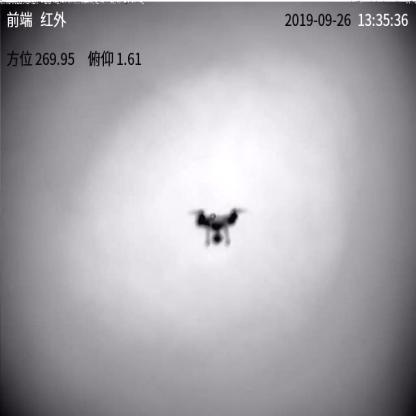
\includegraphics[width=0.9\linewidth]{inv1.JPG}
		\caption{Inversion处理示例}
		\label{txzq21}%文中引用该图片代号
	\end{minipage}
	%\qquad
	%让图片换行,
	
	\begin{minipage}{0.49\linewidth}
		\centering
		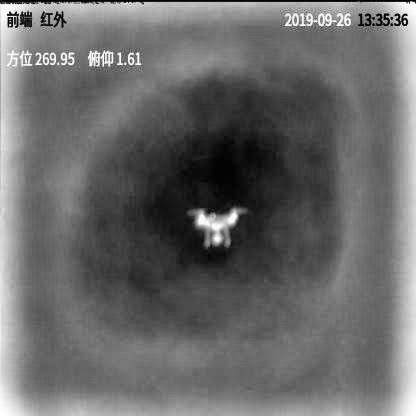
\includegraphics[width=0.9\linewidth]{clahe1.JPG}
		\caption{CLAHE处理示例}
		\label{txzq31}%文中引用该图片代号
	\end{minipage}
	\begin{minipage}{0.49\linewidth}
		\centering
		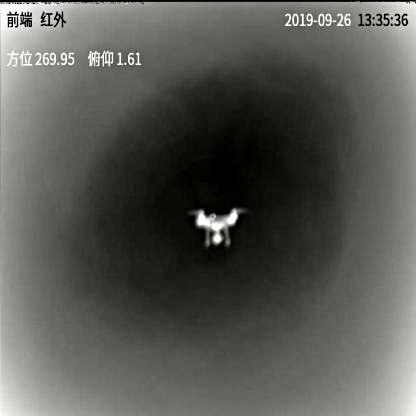
\includegraphics[width=0.9\linewidth]{usm1.JPG}
		\caption{USM处理示例}
		\label{txzq41}%文中引用该图片代号
	\end{minipage}
  \label{txzq}
\end{figure}

增强后的图片效果如图\ref{txzq11}、\ref{txzq21}、\ref{txzq31}、\ref{txzq41}所示,其中\ref{txzq11}表示原图像,\ref{txzq21}表示原图经过Inversion处理后的图像,\ref{txzq31}表示原图像经过CLAHE处理后的图像,\ref{txzq41}表示原图像经过USM处理后的图像。

\subsection{图像拼接算法}
由于在红外无人机目标检测的场景下,无人机目标往往可能从探测器的各方向出现,目标的背景变化较多,因此考虑采用一种图像拼接的数据增强算法,将训练数据中的目标数增多,同时丰富训练数据图像中的背景,增强模型的泛化能力,从而增强网络对目标的检测能力。

该算法的实现方法是,从训练集中随机抽取4个图像,将这4张图像进行拼接后生成一张与原始图像相同大小的新图像输入网络。

\begin{figure}[htbp]
	\centering
	\begin{minipage}{0.49\linewidth}
		\centering
		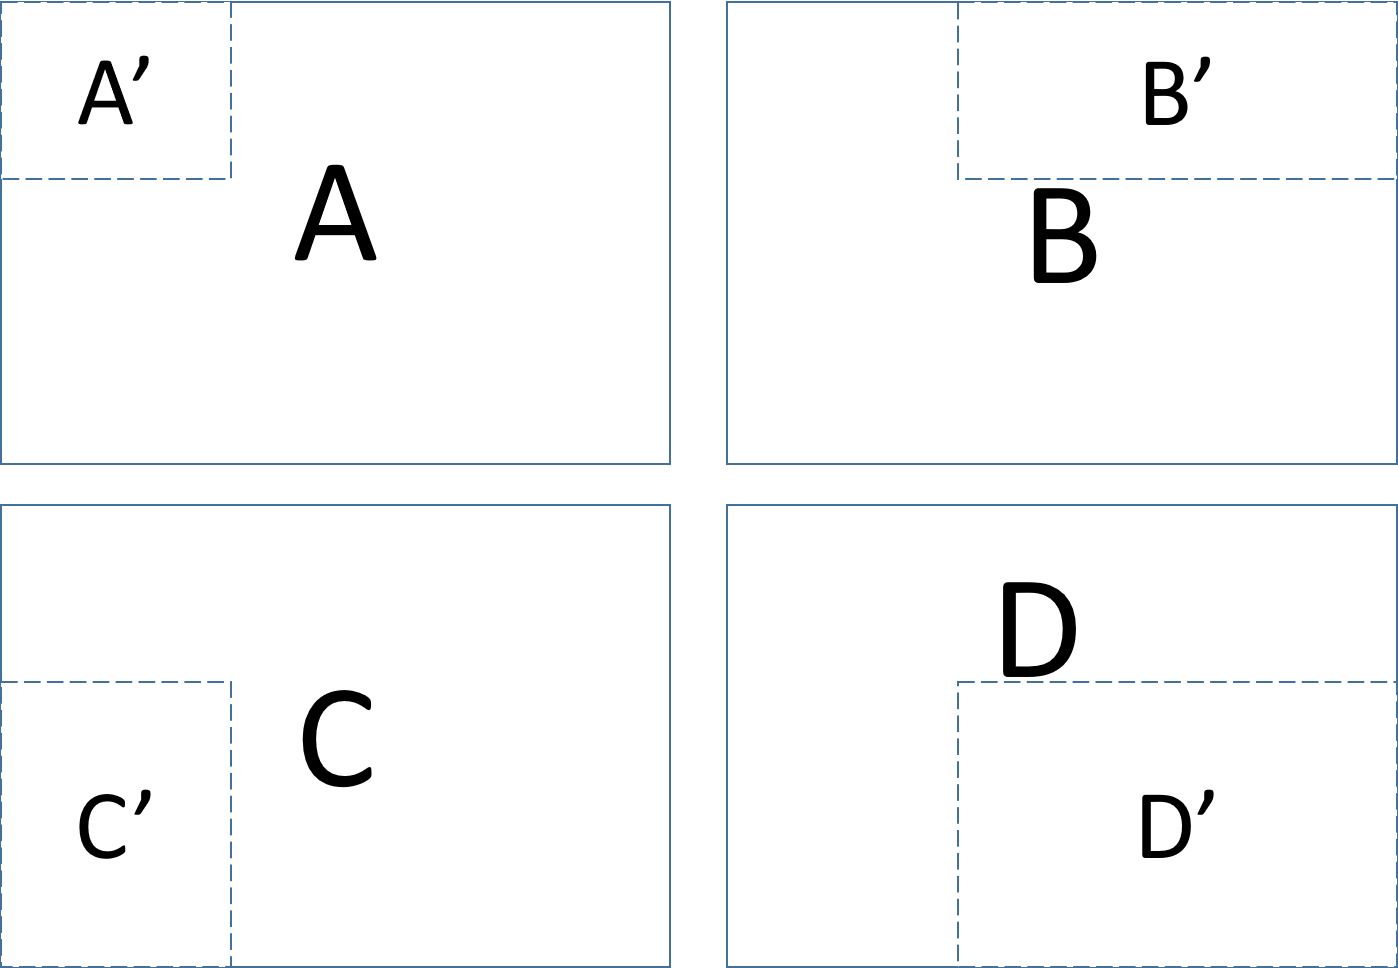
\includegraphics[width=0.9\linewidth]{txpj1.PNG}
		\caption{原始图像及切割示意图}
		\label{txpj1}%文中引用该图片代号
	\end{minipage}
	%\qquad
	\begin{minipage}{0.49\linewidth}
		\centering
		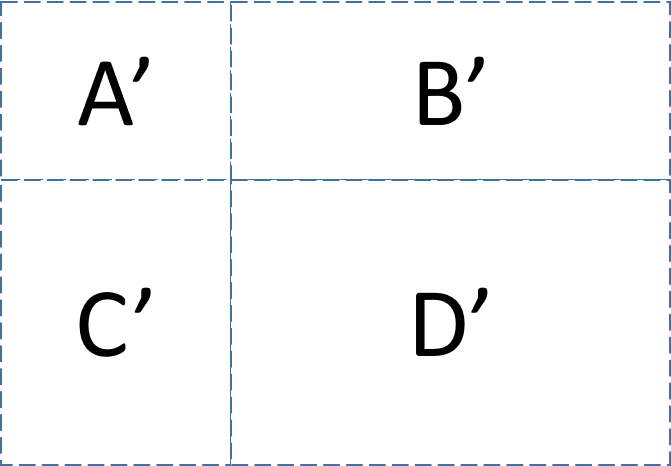
\includegraphics[width=0.9\linewidth]{txpj2.PNG}
		\caption{拼接结果图}
		\label{txpj2}%文中引用该图片代号
	\end{minipage}
\end{figure}

如图\ref{txpj1}所示,图像拼接算法的实现流程是:

(1)图中A、B、C、D分别是4张大小尺寸相同的原始图像,假设长为$w$,宽为$h$。

(2)在图像矩形的中心区域范围内随机生成一个坐标作为四张图片的切割点(例如生成点坐标为$(x,y)$,则限制其中$x\in[0.4w,0.7w],y\in[0.4h,0.7h]$)。

(3)将每张图片分割成四个矩形后,取每张图片的不同部分,即在图A中取A'(原图A的左上部分),在图B中取B'(原图B的右上部分),在图C中取C'(原图C的左下部分),在图D中取D'(原图D的右下部分)。

(4)将4张小图按其在原图中的位置放置后得到结果图,如图\ref{txpj2}所示。

如图\ref{txpj}所示,对随机4张红外无人机数据图像应用图像拼接算法后得到一张包含更丰富背景、更多标注目标的训练样本图。

\begin{figure}[htpb]
  \centering
  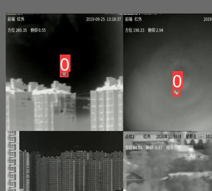
\includegraphics[width = 0.5\textwidth]{图像拼接1.png}
  \caption{图像拼接效果图}
  \label{txpj}
\end{figure}

\section{改进损失函数}
YOLOv5网络的损失函数主要由三部分组成:第一部分是bounding box损失,主要根据预测目标框和真值目标框的重合程度进行计算。第二部分是置信度损失,第三部分是分类误差。

其中对于bounding box的损失函数主要是基于$IoU$(交并比,Intersection over Union)进行计算。$IoU$一般表示预测框与真值框面积的交并比,即二者相交的面积除以二者所占的总面积。
\begin{equation}
  I o U=\frac{|A \cap B|}{|A \cup B|}
\end{equation}

这样一种计算方式相对于之前的基于点到点之间距离的MSE损失函数已经有较大的优势,主要体现在:

(1)MSE损失函数由于是按点距离计算,因此对于任务目标的尺寸变化较为敏感,尺寸变化往往会引起损失函数的无意义波动。

(2)MSE损失函数从点距离出发,忽略了目标框各点之间的关联。因此基于$IoU$的损失函数已经在一定程度上反映了预测框与真值框之间的误差关系。

而$IoU$损失函数有两个重要特性,使得它能作为很多计算机视觉算法的损失函数。

(1)$\mathcal{L}=1-IoU$满足非负性、同一性、对称性、三角不等性等所有损失函数的特性。

(2)$IoU$相对于问题的规模是不变的。这意味着两个任意形状之间的相似性独立于它们的空间规模。

然而基于$IoU$的损失函数也存在一定的问题。

(1)当预测框与真值框没有相交区域时,$IoU$值为0,此时损失loss为0,无法进行梯度回传,也就是无法进行模型训练。

(2)$IoU$还是无法精确地衡量预测框与真值框之间的误差情况,尤其是在$IoU$为0时,预测框与真实框之间的距离变得无法量化。

因此,针对$IoU$的这一问题,为了增强算法对红外无人机目标检测任务中的目标框定位能力,可以引入一种更加完善的$GIoU$损失函数。设$I o U=\frac{\mathcal{I}}{\mathcal{U}}$
,其中$\mathcal{I}$表示预测框与真值框相交部分面积,$\mathcal{U}$表示预测框与真值框合并部分面积,则$GIoU$的计算公式是:
\begin{equation}
  G I o U=I o U-\frac{A^{c}-\mathcal{U}}{A^{c}}
\end{equation}

其中$A^{c}$表示预测框和真值框的最小闭包区域的面积。

\begin{figure}[htbp]
  \centering
  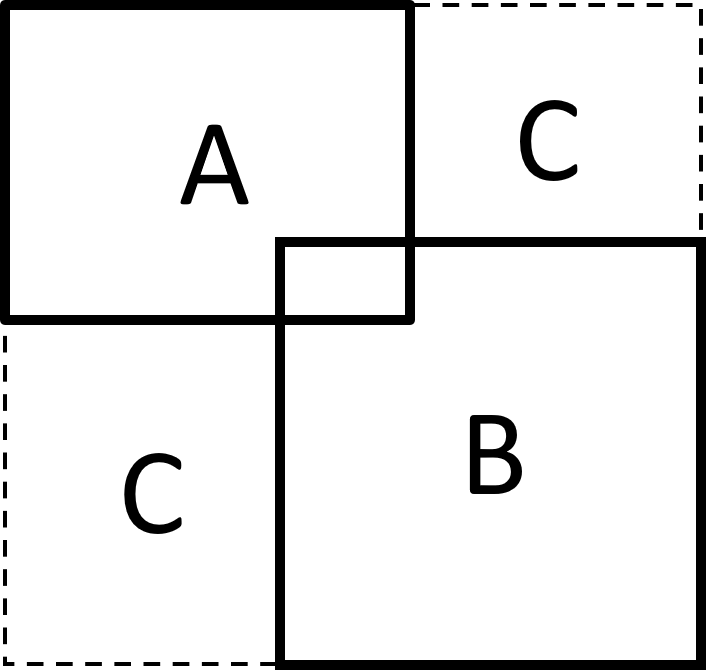
\includegraphics[width = 0.5\textwidth]{giou示意.png}
  \caption{GIoU示意图}
  \label{gi}
\end{figure}

如图\ref{gi}所示,$GIoU$的计算流程是:

(1)找到预测框(图\ref{gi}中区域A)和真值框(图\ref{gi}中区域B)的边界点,计算闭包区域(图\ref{gi}中整个虚线包围的矩形区域)面积。

(2)计算预测框和真值框相交部分和合并部分面积,求得补集部分(图\ref{gi}中区域C)面积。

(3)代入公式$G I o U=I o U-\frac{A^{c}-\mathcal{U}}{A^{c}}$以及$\mathcal{L}_{G I o U}=1-G I o U$得到$\mathcal{L}_{G I o U}$。

$GIoU$是经过改进的$IoU$计算方法,有如下几个特点:

(1)与$IoU$相似,也是一种距离度量,作为损失函数满足损失函数的需求。

(2)$GIoU$除了关注重叠区域不同,还关注了非重叠区域,能够更好的反应重合度。

(3)$GIoU$对目标的尺度不敏感。

(4)当预测框与真值框重合时,$GIoU=IoU$,即$GIoU$的上限是$IoU$,因此训练时不会出现梯度爆炸的情况。

\section{实验结果与分析}
本节将在YOLOv5网络的基础上,应用本章提出的数据增强算法以及损失函数的改进方案,在红外图像无人机目标数据集上进行性能测试和对比,并对实验结果进行分析。


\subsection{实验环境与参数}
本章提到的算法用深度学习网络框架Pytorch进行实现、训练和测试。操作系统为Windows 10,使用的主要软件为python。实验平台采用的CPU型号为Intel Core i7-11700k,GPU型号为NVIDIA GeForce RTX 3080Ti,显存容量为12GB。训练过程中使用GPU进行加速。

\subsection{不同算法对比与分析}
在上述环境下,进行算法的训练和测试,以mAP和推理时间作为评价指标,对比结果列在表\ref{m1}中。

\begin{table}[htbp]
  \caption{不同算法对红外无人机数据集的检测结果}
  \vspace{0.5em}\centering\wuhao
  \begin{tabular}{cc}
  \toprule
  检测算法 & mAP\\
  \midrule
  YOLOv5 & 0.919\\
  Ours(YOLOv5+Inversion数据增强) & 0.924\\
  Ours(YOLOv5+CLAHE数据增强) & 0.918\\
  Ours(YOLOv5+USM数据增强) & 0.913\\
  Ours(YOLOv5+Inversion+CLAHE通道填充) & 0.930\\
  Ours(YOLOv5+Inversion+USM通道填充) & 0.913\\
  Ours(YOLOv5+CLAHE+USM通道填充) & 0.910\\
  Ours(YOLOv5+Inversion+CLAHE通道填充+图像拼接) & 0.929\\
  Ours(YOLOv5+Inversion+CLAHE通道填充+GIoU) & 0.932\\
  Ours(YOLOv5+Inversion+CLAHE通道填充+图像拼接+GIoU) & 0.937\\
  \bottomrule
  \end{tabular}
  \label{m1}
\end{table}

由表\ref{m1}中所示数据可以看出,YOLOv5目标检测算法在本文的检测任务中已经能取得较好的精度。本节首先对基础的数据增强方法进行了对比实验(即对训练数据采用Inversion变换、CLAHE变换、USM变换其中之一处理后生成训练数据)。实验结果显示,在进行Inversion数据增强后,YOLOv5算法的检测精度得到了小幅度的提升,这是由于部分图像在经过Inversion后和原始图像相差较大,使得网络学习到了更为丰富的特征。而应用CLAHE数据增强方法后算法的检测精度基本不变,应用USM数据增强方法后算法的检测精度略有下降,这是因为USM虽然在一定程度上抑制噪声,但是由于有些图像本身的信噪比不高,有相当数量的图像经过USM后增强了噪声,影响了模型的训练效果。随后本节对本文提出的通道填充算法进行了对比实验。实验结果显示,YOLOv5+Inversion+CLAHE通道填充取得了相比于单纯应用Inversion数据增强后的YOLOv5网络取得了更高的检测精度,这是因为网络在经过不同的三通道数据进行训练后增强了特征提取的能力。在应用了图像拼接算法后,算法的精度并没有提高,虽然理论上模型对复杂背景的检测能力得到增强,但是本文采用的训练集已经包含了大量的复杂背景样本,因此单纯应用图像拼接后会使得背景的干扰强度过大,可能一定程度上降低了模型的泛化能力。而后本节对应用了GIoU损失函数的网络结构进行了对比实验,结果显示YOLOv5+Inversion+CLAHE通道填充+图像拼接+GIoU的红外无人机目标检测算法取得了比其他算法更高的检测精度,这一方面是因为GIoU损失函数的改进提高了网络对于目标预测框的定位能力,另一方面是因为图像拼接后,目标框和预测框更容易出现更大的偏差,原始的IoU损失函数性能下降,因此图像拼接算法在配合GIoU损失函数后表现出了更高的检测精度。

\section{本章小结}
本章首先介绍了本文采用的自建红外无人机目标数据集的制作过程。之后本章介绍了本文采用的目标检测算法基于的YOLOv5神经网络的结构,并且在数据集上进行了对比实验,证明了在红外无人机目标检测任务中,YOLOv5算法的检测能力强于常见的YOLOv3算法、Faster-RCNN算法以及SSD算法。此后本章分析了本课题主要面临的问题,其一是本课题的目标检测应用场景是红外图像,其二是无人机目标检测场景下待测目标常常处于复杂背景中。针对这两个问题本章提出了一种数据增强算法,即在训练过程中通过特定的图像处理方法增强模型的训练效果,并且进行了对比试验,验证了对模型的改进效果。此外本章对YOLOv5采用的bbox损失函数进行了改进,进一步增强了本文提出算法在红外无人机数据集上的检测精度。









% Local Variables:
% TeX-master: "../main"
% TeX-engine: xetex
% End:
